\documentclass{beamer}
\usepackage[UKenglish]{babel}
\usepackage[UKenglish]{isodate}
\usepackage{graphicx}
\usepackage{tikz}
\usepackage{bm}
\usepackage{bbm}
\usepackage{mathtools}

\usetheme{SaintPetersburg}
\beamertemplatenavigationsymbolsempty
\usetikzlibrary{shapes,bayesnet}
\newtheorem{proposition}{Proposition}
\DeclareMathOperator*{\argmax}{arg\,max}
\DeclareMathOperator{\diag}{diag}
\DeclareMathOperator{\tr}{tr}
\newcommand{\Kuu}{\mathbf{K}_{\mathbf{u},\mathbf{u}}}
\newcommand{\Krr}{\mathbf{K}_{\mathbf{r},\mathbf{r}}}
\newcommand{\Kru}{\mathbf{K}_{\mathbf{r},\mathbf{u}}}
\newcommand{\rinf}{\lVert \mathbf{r} \rVert_\infty}
\newcommand{\vbound}{\frac{\rinf + \log|\mathcal{A}|}{1 - \gamma}}
\newcommand{\dt}{\frac{\partial}{\partial t}}
\newcommand{\dx}{\,d\mathbf{r}\,d\mathbf{u}}

\DeclarePairedDelimiterX{\infdivx}[2]{(}{)}{%
  #1\;\delimsize\|\;#2%
}
\newcommand{\DKL}{D_{\mathrm{KL}}\infdivx}

\author{Paulius Dilkas}
\title{Variational Inference for Inverse Reinforcement Learning with Gaussian
  Processes}
\date{15th January 2019}

\begin{document}
\maketitle

\begin{frame}{Markov Decision Process}
  \begin{minipage}[t][0.85\textheight]{\textwidth}
    $\mathcal{M} = (\mathcal{S}, \mathcal{A}, \mathcal{T}, \gamma, \mathbf{r})$,
    where
  
    $\mathcal{T} : \mathcal{S} \times \mathcal{A} \times \mathcal{S} \to [0,
    1]$, and

    $\mathbf{r} \in \mathbb{R}^{|\mathcal{S}|} \text{ or } r : \mathcal{S} \to
    \mathbb{R}$.
    \begin{tikzpicture}[state/.style={rectangle, draw, scale=1.5},
      action/.style={diamond, draw, fill=lightgray}, overlay, shift={(-2, -3)}]
      \node(origin) at (0, 0){};
      \node[state](s0) at (1, 0){$s_0$};
      \node[action](start) at (2.5, 0){start};
      \node[state,label=try](s1) at (4, 0){$s_1$};
      \node[action](wait) at (4, -2){wait};
      \node[action](send) at (5.5, 0){send};
      \node[state,label={right:failure},label={below:\textcolor{red}{-1}}](s2) at (7, 2){$s_2$};
      \node[action](restart) at (7, 4){restart};
      \node[state,label={left:success},label={above:\textcolor{green}{+3}}](s3) at (7, -2){$s_3$};
      \node[action](stop) at (8.5, -2){stop};
      \draw[->] (s0) edge (start);
      \draw[->] (start) edge node[above] {$1$} (s1);
      \draw[->,bend left] (s1) edge (wait);
      \draw[->,bend left] (wait) edge node[left] {$1$} (s1);
      \draw[->] (s1) edge (send);
      \draw[->] (send) edge node[left] {$0.01$} (s2);
      \draw[->] (send) edge node[left] {$0.99$} (s3);
      \draw[->] (s2) edge (restart);
      \draw[->,bend right] (restart) edge node[above] {$1$} (s0);
      \draw[->,bend left] (s3) edge (stop);
      \draw[->,bend left] (stop) edge node[below] {$1$} (s3);
      \draw[->] (origin) edge (s0);
    \end{tikzpicture}
    \vfill
    {\hfill\tiny\color{gray}Source: P. Dilkas. Nondeterministic Bigraphs and Their Use
      in Modelling Movement. 2018}
  \end{minipage}
\end{frame}

\begin{frame}{Inverse Reinforcement Learning (COLT 1998)}
  \begin{figure}
    \centering
    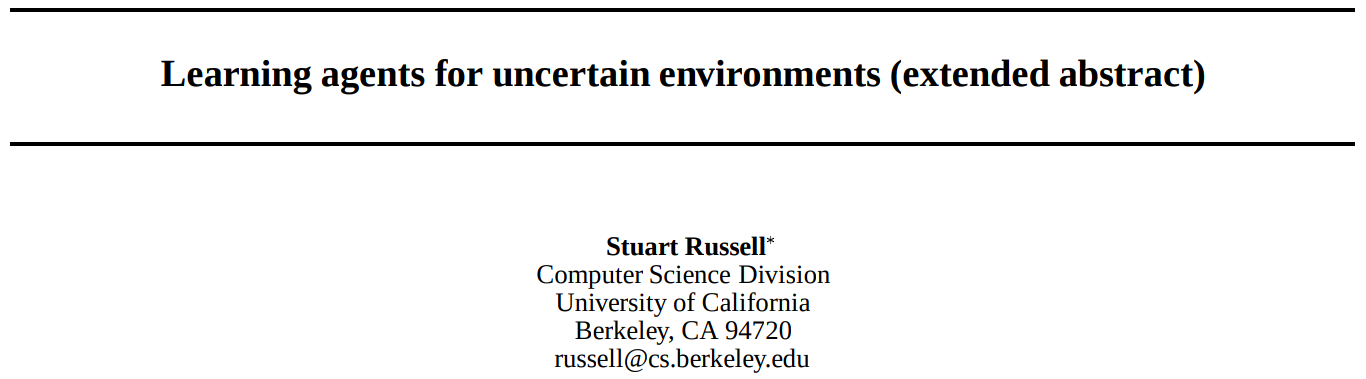
\includegraphics[width=\textwidth]{russell.png}
  \end{figure}
  \begin{tikzpicture}[overlay, shift={(10, 1.8)}]
    \node {
\includegraphics{russell.jpg}};
  \end{tikzpicture}
  \begin{block}{Inverse Reinforcement Learning Problem}
    Given:
    \begin{itemize}
    \item $\mathcal{M} \setminus \{ \mathbf{r} \}$,
    \item $\mathcal{D} = \{ \zeta_i \}_{i=1}^N$, where $\zeta_i = \{ (s_{i,1},
      a_{i,1}), \dots, (s_{i,T}, a_{i,T}) \}$,
    \item features $\mathbf{X} \in \mathbb{R}^{|\mathcal{S}| \times d}$,
    \end{itemize}
    find $\mathbf{r}$.
  \end{block}
\end{frame} % TODO: motivation for solving this

\begin{frame}{Value Iteration}
  \begin{block}{Standard MDP}
    \[
      V_{\mathbf{r}}(s) \coloneqq r(s) + \gamma \max_{a \in \mathcal{A}} \sum_{s' \in
        \mathcal{S}} \mathcal{T}(s, a, s')V_{\mathbf{r}}(s')
    \]
  \end{block}
  \begin{block}{Linearly Solvable / Maximum Causal Entropy MDP}
    \[
      V_{\mathbf{r}}(s) \coloneqq \log \sum_{a \in \mathcal{A}} \exp \left( r(s) +
        \gamma\sum_{s' \in \mathcal{S}} \mathcal{T}(s, a, s')V_{\mathbf{r}}(s')
      \right)
    \]
  \end{block}
\end{frame}

\begin{frame}{Under the Maximum Entropy Model...}
  \[
    p(\mathcal{D} \mid \mathbf{r}) = \prod_{i=1}^N \prod_{t=1}^T p(a_{i,t} \mid
    s_{i,t}) = \exp\left( \sum_{i=1}^N \sum_{t=1}^T Q_{\mathbf{r}}(s_{i,t},
      a_{i,t}) - V_{\mathbf{r}}(s_{i,t}) \right)
  \]
  where
  \[
    Q_{\mathbf{r}}(s, a) = r(s) + \gamma \sum_{s' \in \mathcal{S}}
    \mathcal{T}(s, a, s')V_{\mathbf{r}}(s')
  \]
\end{frame}

\begin{frame}{Reward Function as a Gaussian Process}
  \begin{block}{Automatic Relevance Determination Kernel}
    For any two states $\mathbf{x}_i, \mathbf{x}_j \in \mathbb{R}^d$,
    \[
      k_{\bm\lambda}(\mathbf{x}_i, \mathbf{x}_j) = \lambda_0\exp\left(
        -\frac{1}{2}(\mathbf{x}_i - \mathbf{x}_j)^\intercal\bm\Lambda(\mathbf{x}_i -
        \mathbf{x}_j) - \mathbbm{1}[i \ne j]\sigma^2\tr(\bm\Lambda) \right)
    \]
    where $\bm\Lambda = \diag(\lambda_1, \dots, \lambda_d)$, $\sigma^2 =
    10^{-2}/2$,
    \[
      \mathbbm{1}[b] = \begin{cases}
        1 & \mbox{if $b$ is true} \\
        0 & \mbox{otherwise}.
      \end{cases}
    \]
  \end{block}
\end{frame}

\begin{frame}{Reward Function as a Gaussian Process}
    \begin{block}{Inducing Points}
      \begin{itemize}
      \item $m \ll |\mathcal{S}|$ states,
      \item their features $\mathbf{X_u}$
      \item and rewards $\mathbf{u}$.
      \end{itemize}
    \end{block}

  \begin{block}{The GP Then Gives Gives...}
    \begin{itemize}
    \item Kernel/covariance matrices: $\Kuu$, $\Kru$, $\Krr$
    \item Prior probabilities:
      \begin{itemize}
      \item $p(\mathbf{u}) = \mathcal{N}(\mathbf{u}; \mathbf{0}, \Kuu)$
      \item $p(\mathbf{r} \mid \mathbf{u}) = \mathcal{N}(\mathbf{r};
        \Kru^\intercal\Kuu^{-1}\mathbf{u}, \Krr - \Kru^\intercal\Kuu^{-1}\Kru)$
      \end{itemize}
    \end{itemize}
  \end{block}
\end{frame}

% TODO: why use VI on this problem?

\begin{frame}{Variational Inference}
  \begin{block}{Previous Work}
    \begin{itemize}
    \item Levine et al. (2011) assume that $\mathbf{r} =
      \Kru^\intercal\Kuu^{-1}\mathbf{u}$ and maximise the likelihood
    \item Jin et al. (2017) add more assumptions and use a deep GP model
    \item Wulfmeier et al. (2015) use a neural network
    \end{itemize}
  \end{block}
  What about posterior probabilities?
  \[
    p(\mathbf{r}, \mathbf{u} \mid \mathcal{D}) = \frac{p(\mathcal{D} \mid
      \mathbf{r})p(\mathbf{r} \mid \mathbf{u})p(\mathbf{u})}{p(\mathcal{D})}
  \]
  Solution: approximate $p(\mathbf{r}, \mathbf{u} \mid \mathcal{D})$ with
  $q(\mathbf{r}, \mathbf{u}) = q(\mathbf{r} \mid \mathbf{u})q(\mathbf{u})$, where
  \begin{itemize}
  \item $q(\mathbf{r} \mid \mathbf{u}) = p(\mathbf{r} \mid \mathbf{u})$
  \item $q(\mathbf{u}) = \mathcal{N}(\mathbf{u}; \bm\mu, \bm\Sigma)$
  \end{itemize}
\end{frame}

% TODO: what parameters are we optimising? Maybe add the integral form as well
\begin{frame}{Variational Inference}
  \begin{figure}
    \centering
    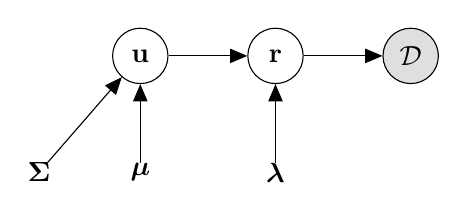
\begin{tikzpicture}
      \node[latent] (u) {$\mathbf{u}$};
      \node[latent, right=of u] (r) {$\mathbf{r}$};
      \node[obs, right=of r] (D) {$\mathcal{D}$};
      \node[const, below=of r] (lambda) {$\bm\lambda$};
      \node[const, below=of u] (mu) {$\bm\mu$};
      \node[const, left=of mu] (Sigma) {$\bm\Sigma$};
      \edge {mu, Sigma} {u};
      \edge {lambda, u} {r};
      \edge {r} {D};
    \end{tikzpicture}
  \end{figure}
  Goal: \alert{minimise} the \emph{Kullback-Leibler divergence}:
  \[
    \begin{split}
      \DKL{q(\mathbf{r}, \mathbf{u})}{p(\mathbf{r}, \mathbf{u} \mid \mathcal{D})}
      &= \mathbb{E}_{(\mathbf{r}, \mathbf{u}) \sim q(\mathbf{r}, \mathbf{u})}[\log
      q(\mathbf{r}, \mathbf{u}) - \log p(\mathbf{r}, \mathbf{u} \mid
      \mathcal{D})] \\
      &= \mathbb{E}_{(\mathbf{r}, \mathbf{u}) \sim q(\mathbf{r},
        \mathbf{u})}[\log q(\mathbf{r}, \mathbf{u}) - \log p(\mathcal{D},
      \mathbf{r}, \mathbf{u})] \\
      &+ \mathbb{E}_{(\mathbf{r}, \mathbf{u}) \sim q(\mathbf{r},
        \mathbf{u})}[\log p(\mathcal{D})]
    \end{split}
  \]
  Equivalently, \alert{maximise} the \emph{evidence lower bound}:
  \[
    \mathcal{L} = \mathbb{E}_{(\mathbf{r}, \mathbf{u}) \sim q(\mathbf{r},
      \mathbf{u})}[\log p(\mathcal{D}, \mathbf{r}, \mathbf{u}) - \log
    q(\mathbf{r}, \mathbf{u})]
  \]
\end{frame}

\begin{frame}{Mathematical Preliminaries}
  \begin{table}
    \centering
    \begin{tabular}{cc}
      Vector norms & Matrix norms \\
      {$\!\begin{aligned}
          \lVert \mathbf{x} \rVert_1 &= \sum_i |x_i| \\
          \lVert \mathbf{x} \rVert_\infty &= \max_i |x_i|
        \end{aligned}$} & {$\!\begin{aligned}
          \lVert \mathbf{A} \rVert_p &= \sup_{\mathbf{x} \ne \mathbf{0}} \frac{\lVert \mathbf{Ax} \rVert_p}{\lVert \mathbf{x} \rVert_p} \\
          \lVert \mathbf{A} \rVert_\infty &= \max_i \sum_{j} |A_{i,j}|
        \end{aligned}$}
    \end{tabular}
  \end{table}
  \begin{lemma}[Perturbation Lemma]
    Let $\lVert \cdot \rVert$ be any matrix norm, and let $\mathbf{A}$ and
    $\mathbf{E}$ be matrices such that $\mathbf{A}$ is invertible and $\lVert
    \mathbf{A}^{-1} \rVert \lVert \mathbf{E} \rVert < 1$, then $\mathbf{A} +
    \mathbf{E}$ is invertible, and
    \[
      \lVert (\mathbf{A} + \mathbf{E})^{-1} \rVert \le \frac{\lVert
        \mathbf{A}^{-1} \rVert}{1 - \lVert \mathbf{A}^{-1} \rVert \lVert
        \mathbf{E} \rVert}.
    \]
  \end{lemma}
\end{frame}

\begin{frame}{Theoretical Results}
  Seeing $V$ as $V : \mathcal{S} \to \mathbb{R}^{|\mathcal{S}|} \to
  \mathbb{R}$... \\~\\

  \begin{proposition}
    MDP value functions $V(s) : \mathbb{R}^{|\mathcal{S}|} \to \mathbb{R}$ (for
    $s \in \mathcal{S}$) are Lebesgue measurable.
  \end{proposition}
  \begin{proposition}
    If the initial values of the MDP value function satisfy the following
    bound, then the bound remains satisfied throughout value iteration:
    \[
      |V_{\mathbf{r}}(s)| \le \vbound.
    \]
  \end{proposition}
\end{frame}

\begin{frame}{Theoretical Results}
  \begin{theorem} \label{thm:main}
    Whenever the derivative exists,
    \[
      \dt\iint
      V_{\mathbf{r}}(s)q(\mathbf{r} \mid \mathbf{u})q(\mathbf{u})\dx
      = \iint
      \dt[V_{\mathbf{r}}(s)q(\mathbf{r} \mid \mathbf{u})q(\mathbf{u})]\dx,
    \]
    where $t$ is any scalar part of $\bm\mu$, $\bm\Sigma$, or $\bm\lambda$.
  \end{theorem}
\end{frame}

\begin{frame}{A Note on Polynomials}
  \begin{definition}
    Let $\mathbb{R}_d[\mathbf{x}]$ denote the vector space of polynomials with
    degree at most $d$, where variables are elements of $\mathbf{x}$, and
    coefficients are in $\mathbb{R}$.
  \end{definition}
  \begin{example}
    \[
      \begin{split}
        \mathbb{R}_2[\mathbf{x}] \supset \{ &2x_1^2 + \pi x_2,\\
        &x_1x_2,\\
        &-3x_1 + 1,\\
        &0 \}
      \end{split}
    \]
  \end{example}
\end{frame}

\begin{frame}{Helpful Lemmas}
  \begin{lemma}
    \[
      \int \lVert \mathbf{r} \rVert_\infty q(\mathbf{r} \mid
      \mathbf{u})\,d\mathbf{r} \le a + \lVert \Kru^\intercal \Kuu^{-1}
      \mathbf{u} \rVert_1,
    \]
    where $a$ is a constant independent of $\mathbf{u}$.
  \end{lemma}
  \begin{lemma}
    Let $c : \mathbb{R}^{|\mathcal{S}|} \times \mathbb{R}^m \to (a, b) \subset
    \mathbb{R}$ be an arbitrary bounded function. Then, for $i = 0,
    \dots, d$,
    \[
      \left. \frac{\partial q(\mathbf{r} \mid \mathbf{u})}{\partial \lambda_i}
      \right|_{\lambda_i = c(\mathbf{r}, \mathbf{u})}
    \]
    has upper and lower bounds of the form $q(\mathbf{r} \mid
    \mathbf{u})d(\mathbf{u})$, where $d(\mathbf{u}) \in
    \mathbb{R}_2[\mathbf{u}]$.
  \end{lemma}
\end{frame}

\begin{frame}{Helpful Lemmas}
  \begin{lemma}
    Let $c : \mathbb{R}^{|\mathcal{S}|} \times \mathbb{R}^m \to (a, b) \subset
    \mathbb{R}$ be an arbitrary bounded function. Then, for $i = 1, \dots, m$,
    every element of
    \[
      \left. \frac{\partial q(\mathbf{u})}{\partial \bm\mu} \right|_{\mu_i =
        c(\mathbf{r}, \mathbf{u})}
    \]
    has upper and lower bounds of the form $q(\mathbf{u})d(\mathbf{u})$,
    where $d(\mathbf{u}) \in \mathbb{R}_1[\mathbf{u}]$.
  \end{lemma}
\end{frame}

\begin{frame}{Helpful Lemmas}
  \begin{lemma} \label{lemma:bound3}
    Let $i, j = 1, \dots, m$, and let $\epsilon > 0$ be arbitrary. Furthermore,
    let
    \[
      c : \mathbb{R}^{|\mathcal{S}|} \times \mathbb{R}^m \to (\Sigma_{i,j} - \epsilon,
      \Sigma_{i,j} + \epsilon) \subset \mathbb{R}
    \]
    be a function with a codomain arbitrarily close to $\Sigma_{i,j}$. Then every
    element of
    \[
      \left. \frac{\partial q(\mathbf{u})}{\partial \bm\Sigma} \right|_{\Sigma_{i,j} =
        c(\mathbf{r}, \mathbf{u})}
    \]
    has upper and lower bounds of the form $q(\mathbf{u})d(\mathbf{u})$, where
    $d(\mathbf{u}) \in \mathbb{R}_2[\mathbf{u}]$.
  \end{lemma}
\end{frame}
\end{document}